\section{Vision-and-Language Navigation~\cite{DBLP:journals/corr/abs-1711-07280}}
The idea that they might be able to give general, verbal instructions to a robot and have at least a reasonable probability that it will carry out the required task is one of the long-held goals of robotics, and artificial intelligence (AI). 
Despite significant progress, there are a number of major technical challenges that need to be over come before robots will be able to perform general tasks in the real world. One of the primary requirements will be new techniques for linking natural language to vision and action in \emph{unstructured}, \emph{previously unseen environments}. It is the navigation version of this challenge that we refer to as Vision-and-Language Navigation (VLN)~\cite{DBLP:journals/corr/abs-1711-07280}.

\begin{figure}[htbp]
    \centering
    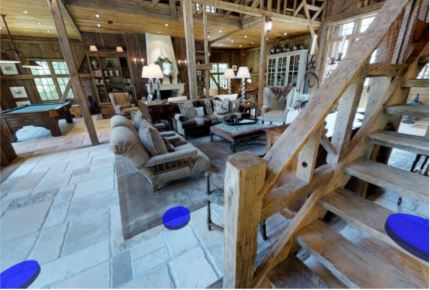
\includegraphics[width=.8\textwidth]{vln}
    \caption{Room-to-Room (R2R) navigation task}
\end{figure}
\newpage
\subsection*{Instruction}
Head upstairs and walk past the piano through an archway directly in front. Turn right when the hallway ends at pictures and table. Wait by the moose antlers hanging on the wall.\\

Previous approaches to natural language command of robots have often neglected the visual information processing aspect of the problem. The R2R dataset is the first dataset to evaluate the capability to follow natural language navigation instructions in previously unseen real images at building scale. To explore this task they investigated several baselines and a sequence-to-sequence neural network agent.  The process used to generate R2R is applicable to a host of related vision and language problems, particularly in robotics. 
